\section{Statistical distributions}
\label{sec:stats_distributions}

We explore a handful of the statistical distributions in
\texttt{scipy.stats} module and the connections between them.  The
organization of the distribution functions in \texttt{scipy.stats} is
quite elegant, with each distribution providing random variates
(\texttt{rvs}), analytical moments (mean, variance, skew, kurtosis),
analytic density (\texttt{pdf}, \texttt{cdf}) and survival functions
(\texttt{sf}, \texttt{isf}) (where available) and tools for fitting
empirical distributions to the analytic distributions (\texttt{fit}).

in the exercise below, we will simulate a radioactive particle
emitter, and look at the empirical distribution of waiting times
compared with the expected analytical distributions.  Our radioative
particle emitter has an equal likelihood of emitting a particle in any
equal time interval, and emits particles at a rate of 20~Hz.  We will
discretely sample time at a high frequency, and record a 1 of a
particle is emitted and a 0 otherwise, and then look at the
distribution of waiting times between emissions.  The probability of a
particle emission in one of our sample intervals (assumed to be very
small compared to the average interval between emissions) is
proportional to the rate and the sample interval $\Delta t$, ie
$p(\Delta t) = \alpha \Delta t$ where $\alpha$ is the emission rate in
particles per second.

\begin{lstlisting}

# a uniform distribution [0..1]
In [62]: uniform = scipy.stats.uniform()

# our sample interval in seconds
In [63]: deltat = 0.001

# the emission rate, 20Hz
In [65]: alpha = 20

# 1000 random numbers
In [66]: rvs = uniform.rvs(1000)

# a look at the 1st 20 random variates
In [67]: rvs[:20]
Out[67]: 
array([ 0.71167172,  0.01723161,  0.25849255,  0.00599207,  0.58656146,
        0.12765225,  0.17898621,  0.77724693,  0.18042977,  0.91935639,
        0.97659579,  0.59045477,  0.94730366,  0.00764026,  0.12153159,
        0.82286929,  0.18990484,  0.34608396,  0.63931108,  0.57199175])

# we simulate an emission when the random number is less than
# p(Delta t) = alpha * deltat
In [84]: emit = rvs < (alpha * deltat)


# there were 3 emissions in the first 20 observations
In [85]: emit[:20]
Out[85]: 
array([False,  True, False,  True, False, False, False, False, False,
       False, False, False, False,  True, False, False, False, False,
       False, False], dtype=bool)
\end{lstlisting}

The waiting times between the emissions should follow an exponential
distribution (see \texttt{scipy.stats.expon}) with a mean of
$1/\alpha$.  In the exercise below, you will generate a long array of
emissions, compute the waiting times between emissions, between 2
emissions, and between 10 emissions.  These should approach an 1st
order gamma (aka exponential) distribution, 2nd order gamma, and 10th
order gamma (see \texttt{scipy.stats.gamma}).  Use the probability
density functions for these distributions in \texttt{scipy.stats} to
compare your simulated distributions and moments with the analytic
versions provided by \texttt{scipy.stats}.  With 10 waiting times, we
should be approaching a normal distribution since we are summing 10
waiting times and under the central limit theorem the sum of
independent samples from a finite variance process approaches the
normal distribution (see \texttt{scipy.stats.norm}).  In the final
part of the exercise below, you will be asked to approximate the 10th
order gamma distribution with a normal distribution.  The results
should look something like those in
Figure~\ref{fig:stats_distributions}.

\lstinputlisting[label=code:stats_distributions_skel,caption={IGNORED}]{skel/stats_distributions_skel.py}

\begin{figure}
\begin{centering}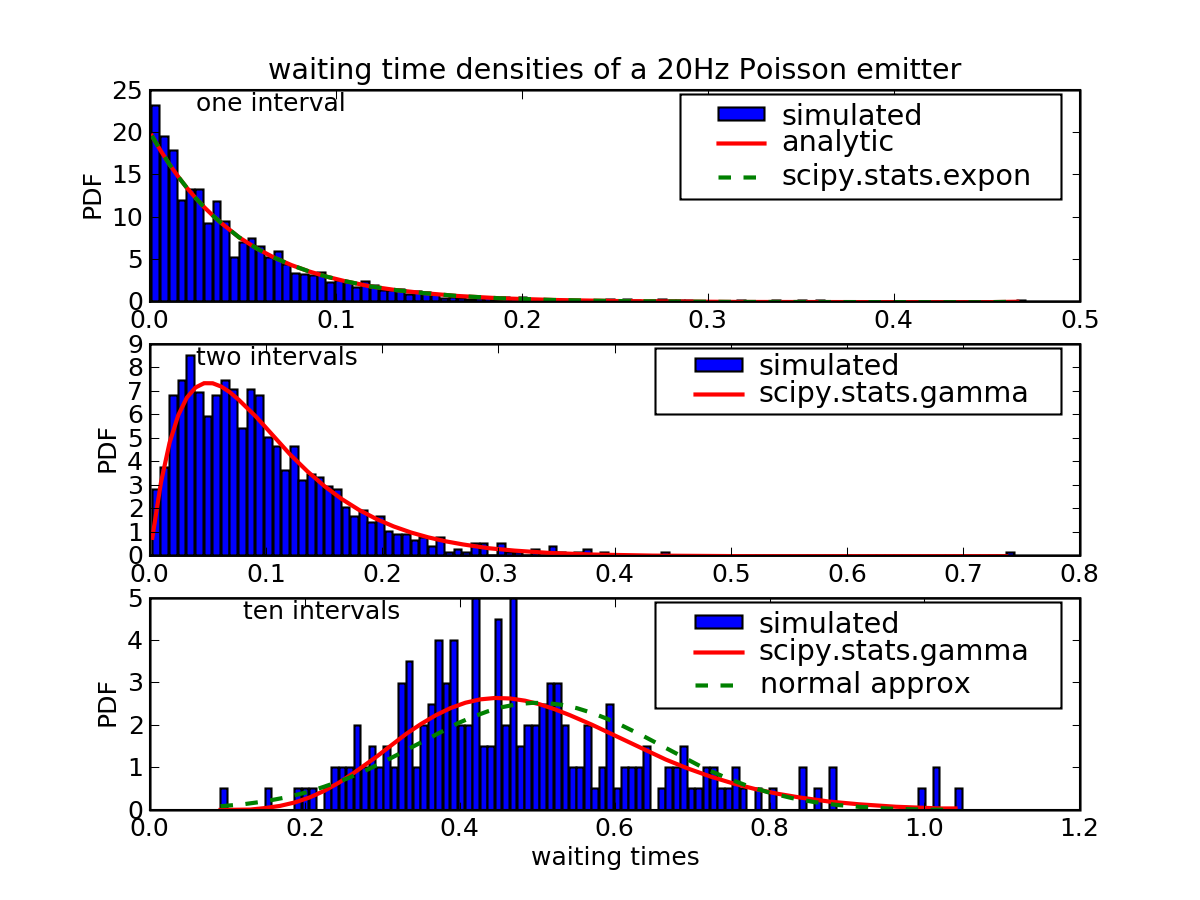
\includegraphics[width=4in]{fig/stats_distributions}\par\end{centering}

\caption{\label{fig:stats_distributions}}
\end{figure}
